\section{Experiment Environment} 
\label{s4:capture}

Load leveling is a system that usually found in renewable sources electricity generator. System’s function is to balance the excess energy, for example in solar panel case; it can either store or sale the excess electricity produced during day time, while discharge electricity during night.

\textbf{eroom} is an IoT system that connects load levelling with battery, control panel, air conditioners and solar panel. The network topology of eroom IoT is shown in figure \ref{fig:s4_eroom}. 

\begin{figure}[H]
    \centering  
    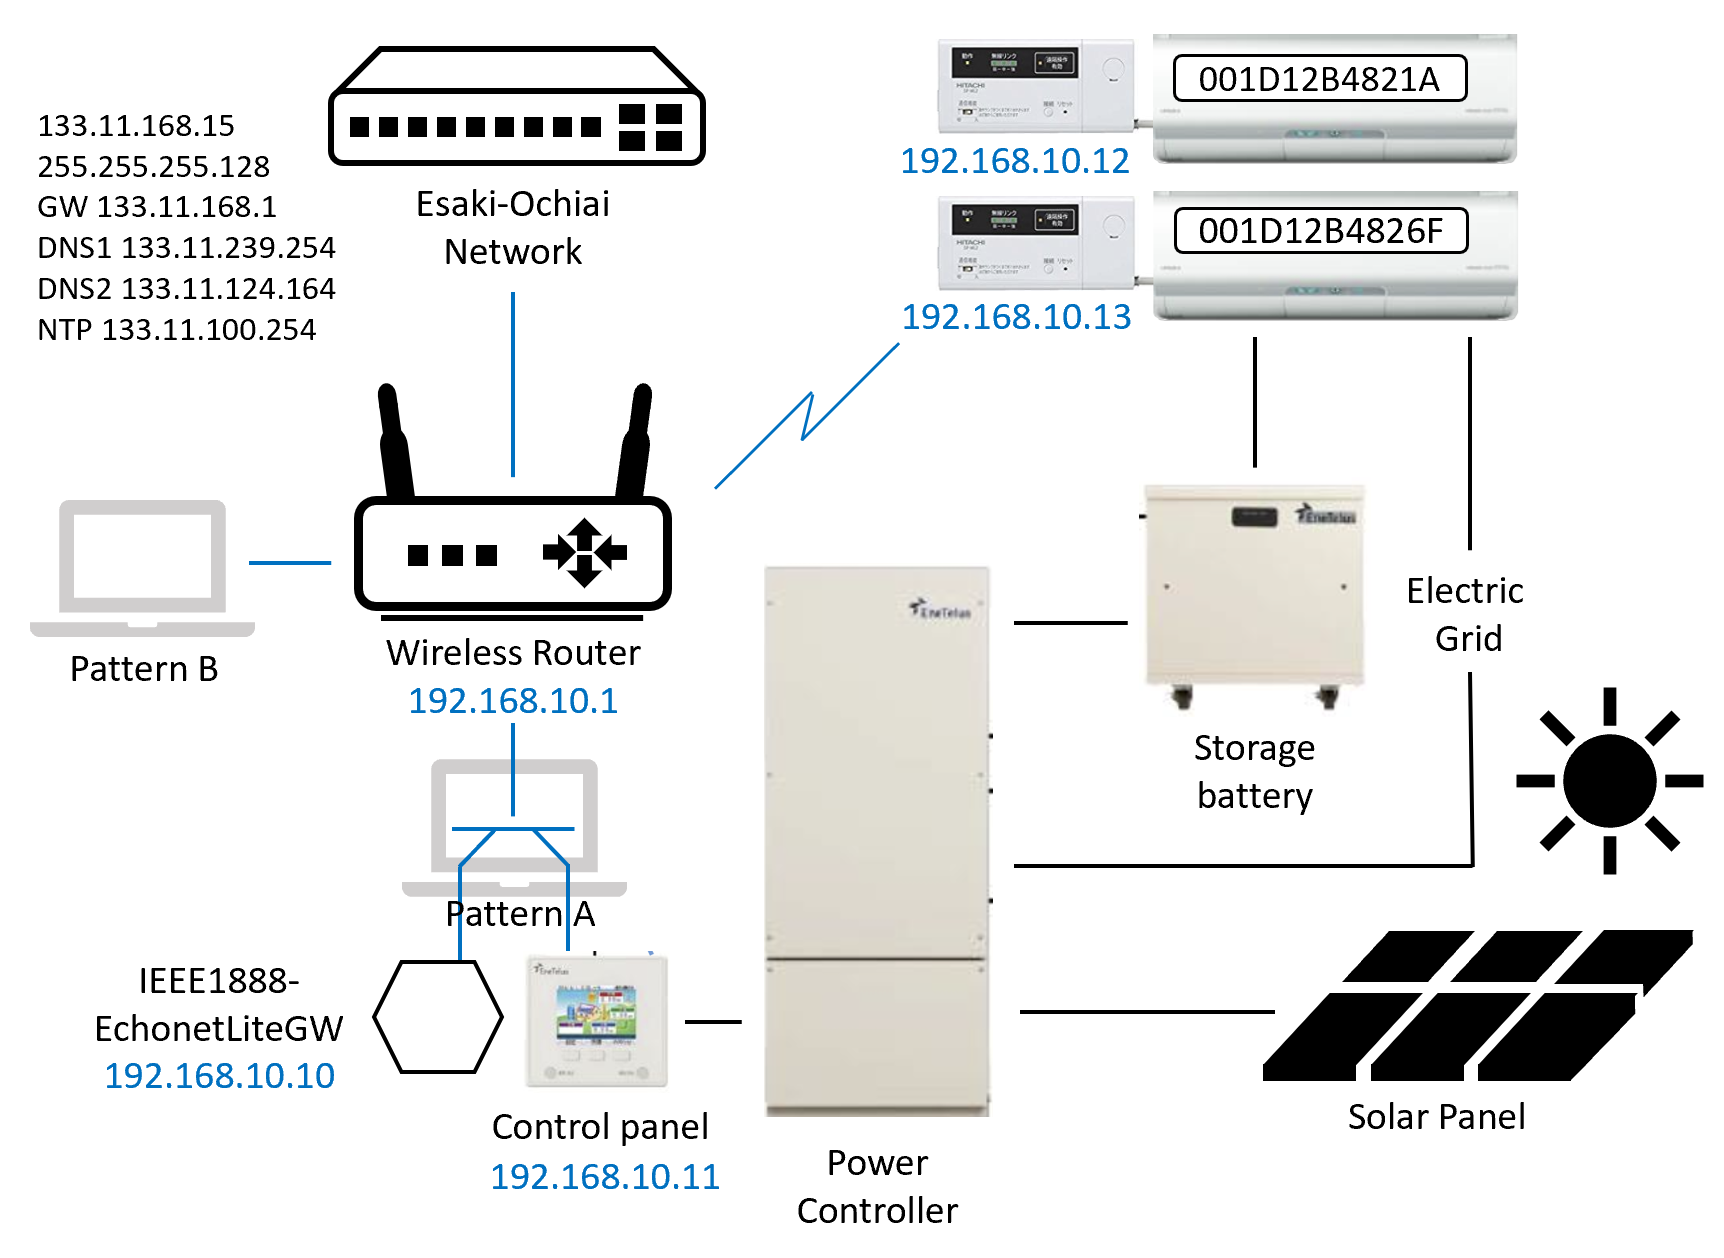
\includegraphics[width=0.8\textwidth]{4_eroom} 
    \caption{\small The network topology of eroom.} 
    \label{fig:s4_eroom} 
\end{figure}  

Blue line indicates that devices is connected through ethernet cable, while black line represents the electrical cable. 
Devices are connected to the internet through the network of Esaki-Ochiai laboratory. 
Electricity produced by the solar cell is sent to the load levelling unit. 
Load levelling unit then provides the necessary energy to the air conditioners,
while stores the excess energy at the battery. 
During night time, when the electricity produced from solar cell is insufficient, 
load leveling can provide the needed electric from battery. 
User can also configure the way load leveling operate through the control panel. 
The consumption data, along with command code is passed to EchoLiteGW for taking record. 

\begin{itemize}[itemsep=0mm] 
    \item The control panel (192.168.10.11). This control panel is used as user interface, it can take command of how load leveling should operate, visualize the collected data: how much electricity has been produced, how much electricity did air conditioner has consumed, and more. 
    \item IEEE1888-EchonetLiteGW (192.168.10.10). EchonetLite is communication protocol standard for smart devices used in house (air conditioner, lighting equipment or electricity sensor). In this IoT system, air conditioner controllers and the control panel communicate with each other using Profinet (UDP/3610), IEEE1888-EchonetLiteGW serves as a gateway adapter, translate Profinet protocol data into XML for storing data on GUTP server.  
    \item 2 Air conditioners with controller (192.168.10.12, 192.168.10.13). This air conditioners are operating according to the setting from the control panel. 
    \item (Wireless Router (192.168.10.1). It is used to connect all 4 devices and the internet) 
\end{itemize} 